% GENERATED from evidence/offline_results/OFFLINE_MECHANISMS_V1.json
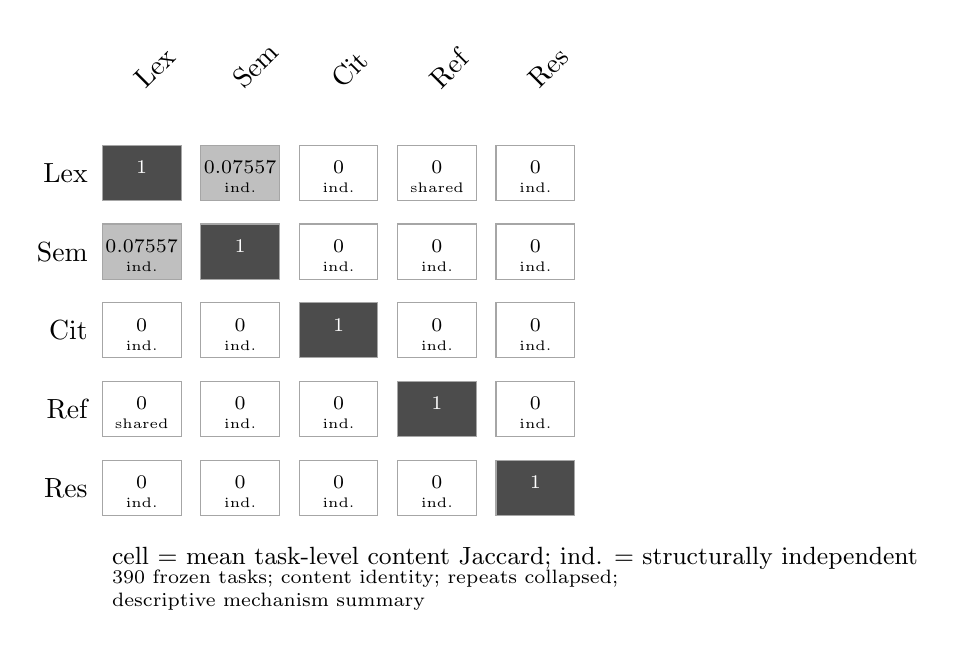
\begin{tikzpicture}[x=1.25cm,y=1.0cm]
\node[rotate=45,anchor=west] at (1,5.4) {Lex};
\node[rotate=45,anchor=west] at (2,5.4) {Sem};
\node[rotate=45,anchor=west] at (3,5.4) {Cit};
\node[rotate=45,anchor=west] at (4,5.4) {Ref};
\node[rotate=45,anchor=west] at (5,5.4) {Res};
\node[anchor=east] at (0.65,4.35) {Lex};
\filldraw[fill=black!70,draw=black!35] (0.70,4.00) rectangle (1.50,4.70);
\node[text=white,font=\scriptsize] at (1.10,4.42) {1};
\filldraw[fill=black!25,draw=black!35] (1.70,4.00) rectangle (2.50,4.70);
\node[text=black,font=\scriptsize] at (2.10,4.42) {0.07557};
\node[text=black,font=\tiny] at (2.10,4.16) {ind.};
\filldraw[fill=white,draw=black!35] (2.70,4.00) rectangle (3.50,4.70);
\node[text=black,font=\scriptsize] at (3.10,4.42) {0};
\node[text=black,font=\tiny] at (3.10,4.16) {ind.};
\filldraw[fill=white,draw=black!35] (3.70,4.00) rectangle (4.50,4.70);
\node[text=black,font=\scriptsize] at (4.10,4.42) {0};
\node[text=black,font=\tiny] at (4.10,4.16) {shared};
\filldraw[fill=white,draw=black!35] (4.70,4.00) rectangle (5.50,4.70);
\node[text=black,font=\scriptsize] at (5.10,4.42) {0};
\node[text=black,font=\tiny] at (5.10,4.16) {ind.};
\node[anchor=east] at (0.65,3.35) {Sem};
\filldraw[fill=black!25,draw=black!35] (0.70,3.00) rectangle (1.50,3.70);
\node[text=black,font=\scriptsize] at (1.10,3.42) {0.07557};
\node[text=black,font=\tiny] at (1.10,3.16) {ind.};
\filldraw[fill=black!70,draw=black!35] (1.70,3.00) rectangle (2.50,3.70);
\node[text=white,font=\scriptsize] at (2.10,3.42) {1};
\filldraw[fill=white,draw=black!35] (2.70,3.00) rectangle (3.50,3.70);
\node[text=black,font=\scriptsize] at (3.10,3.42) {0};
\node[text=black,font=\tiny] at (3.10,3.16) {ind.};
\filldraw[fill=white,draw=black!35] (3.70,3.00) rectangle (4.50,3.70);
\node[text=black,font=\scriptsize] at (4.10,3.42) {0};
\node[text=black,font=\tiny] at (4.10,3.16) {ind.};
\filldraw[fill=white,draw=black!35] (4.70,3.00) rectangle (5.50,3.70);
\node[text=black,font=\scriptsize] at (5.10,3.42) {0};
\node[text=black,font=\tiny] at (5.10,3.16) {ind.};
\node[anchor=east] at (0.65,2.35) {Cit};
\filldraw[fill=white,draw=black!35] (0.70,2.00) rectangle (1.50,2.70);
\node[text=black,font=\scriptsize] at (1.10,2.42) {0};
\node[text=black,font=\tiny] at (1.10,2.16) {ind.};
\filldraw[fill=white,draw=black!35] (1.70,2.00) rectangle (2.50,2.70);
\node[text=black,font=\scriptsize] at (2.10,2.42) {0};
\node[text=black,font=\tiny] at (2.10,2.16) {ind.};
\filldraw[fill=black!70,draw=black!35] (2.70,2.00) rectangle (3.50,2.70);
\node[text=white,font=\scriptsize] at (3.10,2.42) {1};
\filldraw[fill=white,draw=black!35] (3.70,2.00) rectangle (4.50,2.70);
\node[text=black,font=\scriptsize] at (4.10,2.42) {0};
\node[text=black,font=\tiny] at (4.10,2.16) {ind.};
\filldraw[fill=white,draw=black!35] (4.70,2.00) rectangle (5.50,2.70);
\node[text=black,font=\scriptsize] at (5.10,2.42) {0};
\node[text=black,font=\tiny] at (5.10,2.16) {ind.};
\node[anchor=east] at (0.65,1.35) {Ref};
\filldraw[fill=white,draw=black!35] (0.70,1.00) rectangle (1.50,1.70);
\node[text=black,font=\scriptsize] at (1.10,1.42) {0};
\node[text=black,font=\tiny] at (1.10,1.16) {shared};
\filldraw[fill=white,draw=black!35] (1.70,1.00) rectangle (2.50,1.70);
\node[text=black,font=\scriptsize] at (2.10,1.42) {0};
\node[text=black,font=\tiny] at (2.10,1.16) {ind.};
\filldraw[fill=white,draw=black!35] (2.70,1.00) rectangle (3.50,1.70);
\node[text=black,font=\scriptsize] at (3.10,1.42) {0};
\node[text=black,font=\tiny] at (3.10,1.16) {ind.};
\filldraw[fill=black!70,draw=black!35] (3.70,1.00) rectangle (4.50,1.70);
\node[text=white,font=\scriptsize] at (4.10,1.42) {1};
\filldraw[fill=white,draw=black!35] (4.70,1.00) rectangle (5.50,1.70);
\node[text=black,font=\scriptsize] at (5.10,1.42) {0};
\node[text=black,font=\tiny] at (5.10,1.16) {ind.};
\node[anchor=east] at (0.65,0.35) {Res};
\filldraw[fill=white,draw=black!35] (0.70,0.00) rectangle (1.50,0.70);
\node[text=black,font=\scriptsize] at (1.10,0.42) {0};
\node[text=black,font=\tiny] at (1.10,0.16) {ind.};
\filldraw[fill=white,draw=black!35] (1.70,0.00) rectangle (2.50,0.70);
\node[text=black,font=\scriptsize] at (2.10,0.42) {0};
\node[text=black,font=\tiny] at (2.10,0.16) {ind.};
\filldraw[fill=white,draw=black!35] (2.70,0.00) rectangle (3.50,0.70);
\node[text=black,font=\scriptsize] at (3.10,0.42) {0};
\node[text=black,font=\tiny] at (3.10,0.16) {ind.};
\filldraw[fill=white,draw=black!35] (3.70,0.00) rectangle (4.50,0.70);
\node[text=black,font=\scriptsize] at (4.10,0.42) {0};
\node[text=black,font=\tiny] at (4.10,0.16) {ind.};
\filldraw[fill=black!70,draw=black!35] (4.70,0.00) rectangle (5.50,0.70);
\node[text=white,font=\scriptsize] at (5.10,0.42) {1};
\node[anchor=west,font=\small] at (0.7,-0.55) {cell = mean task-level content Jaccard; ind. = structurally independent};
\node[anchor=west,font=\scriptsize,text width=6.8cm,align=left] at (0.7,-0.95) {390 frozen tasks; content identity; repeats collapsed; descriptive mechanism summary};
\end{tikzpicture}
